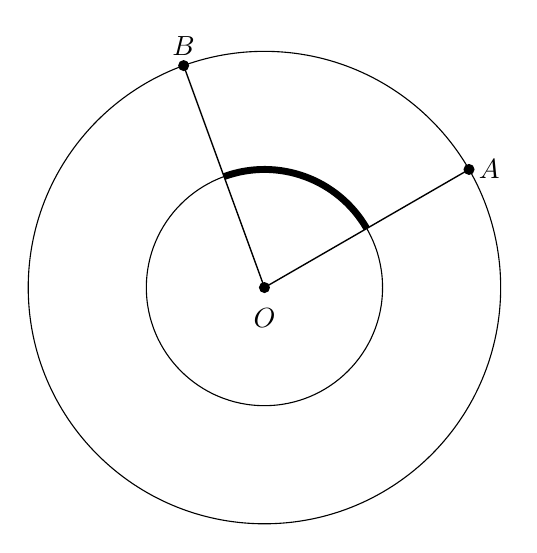
\begin{tikzpicture}[baseline=0]
    % Draw the circles with radii 1.5 and 3
    \draw (0,0) circle (1.5cm);
    \draw (0,0) circle (3cm);
    
    % Define points
    \coordinate (O) at (0,0);
    \coordinate (A) at ({3*cos(30)}, {3*sin(30)});  % First radius, 30 degrees
    \coordinate (C) at ({3*cos(110)}, {3*sin(110)}); % Second radius, 110 degrees
    
    % Calculate intersection points on the smaller circle
    \coordinate (A') at ({1.5*cos(30)}, {1.5*sin(30)}); % Intersection of first radius with smaller circle
    \coordinate (B') at ({1.5*cos(110)}, {1.5*sin(110)}); % Intersection of second radius with smaller circle

    % Draw radius
    \draw[line width=0.5pt] (O) -- (A);
    \draw[line width=0.5pt] (O) -- (C);
    
    % Label the points
    \node at (A) [right] {$A$};
    \node at (C) [above] {$B$};

    % Draw points at the ends of the diameters
    \fill (A) circle (2pt);
    \fill (C) circle (2pt);

    % Mark the center of the circle with a dot
    \fill (O) circle (2pt);
    \node at (O) [below=4pt] {$O$}; % Move the label slightly below
    
    \draw[line width=2.5pt] (A') arc[start angle=30, end angle=110, radius=1.5cm];
\end{tikzpicture}